\documentclass[11pt,oneside,a4paper]{report}
%%%%%%%%%%%%%% General %%%%%%%%%%%%%%%%%%%%%%%


\usepackage[utf8]{inputenc}

%language
\usepackage[portuguese]{babel}

%page layout
\usepackage[a4paper,width=150mm,top=25mm,bottom=25mm]{geometry}

% footers and headers
\usepackage{fancyhdr}
\pagestyle{fancy}

%citations
\usepackage{cite}

%enumerate
\usepackage{enumitem}

%references link
\usepackage{hyperref}

% code input
\usepackage{minted}

%%%%%%%%%%%%%%%% graphicx %%%%%%%%%%%%%%%%%%%%%

\usepackage{graphicx}

\usepackage{tikz,pgfplots}

% include graphics path
\graphicspath{ {images} }
% create external plots
\usepgfplotslibrary{external} 
\tikzexternalize


%%%%%%%%%%%%%%%%%%%%%%%%%%%%%%%%%%%%%%%%%%%%%%%%
%%%%%%%%%%%%%%%% mathematics %%%%%%%%%%%%%%%%%%%%%

\usepackage{mathtools, amsmath}

\DeclareMathOperator{\Tr}{Tr}

% import set notation
\usepackage{amsfonts}

%%%%%%%%%%%%%%%%%%%%%%%%%%%%%%%%%%%%%%%%%%%%%%%%
%%%%%%%%%%%%%%%% notation %%%%%%%%%%%%%%%%%%%%%%

\newcommand{\matriz}[1]{\hat#1}

\newcommand{\many}[2]{$#1_1, #1_2, \dots, #1_#2$}

\newcommand{\cmany}[3]{$#1_1 #3 #1_2 #3 \dots #3 #1_#2$}

\newcommand{\set}[1]{\{#1\}}

%%%%%%%%%%%%%%%%%%%%%%%%%%%%%%%%%%%%%%%%%%%%%%%%%
%%%%%%%%%%%% Theorem %%%%%%%%%%%%%%%%%%%%%%%%%%

\newtheorem{lemma}{Lema}
\newtheorem{theorem}[lemma]{Teorema}
\newtheorem{corolary}[lemma]{Corolário}
\newtheorem{definition}[lemma]{Definição}
\newtheorem{conjecture}[lemma]{Conjectura}
\newtheorem{proposition}[lemma]{Preposição}




% Title Page
\title{
	{No estudo de Matrizes Aleatórias e Simulação de Gases de Coulomb}\\
}
\author{PIMENTA, J. V. A.}


\begin{document}
\maketitle

\begin{abstract}
	Resumo dos estudos de Iniciação Científica em Matrizes Aleatórias e Simulação de Gases de Coulomb.
\end{abstract}

\tableofcontents

\chapter{Introdução}
 Um esquema útil para organização é a classificação de Layman. Denomina-se

\begin{enumerate}
	\item \textbf{Entradas Independentes}: Adicionada a necessidade de simetria, matrizes deste tipo são chamadas matrizes de Wigner.
	\item \textbf{Invariantes por rotação}: Quaisquer duas matrizes que são relacionadas por uma transformação $\matriz{H'} = \matriz{U} \matriz{H} \matriz{U}^{-1}$ ocorrerão com a mesma probabilidade.
\end{enumerate}

Só existe um tipo especial de matriz que se encontra na intersecção e são as classes Gaussianas.

Em geral no mundo das matrizes aleatórias três classes são muito importantes e serão atores centrais no nosso estudo. São as três classes associadas às matrizes que tem entradas gaussianas. Estas são: O Ensemble Gaussiano Ortogonal (GOE), O Ensemble Gaussiano Unitário (GUE) e o Ensemble Gaussiano Simplético (GSE). Em suma, eles tratam, em ordem, de matrizes com entradas gaussianas reais, complexas e quaterniônicas. Seus nomes estão relacionados com a matriz necessária para a transformação de diagonalização das matrizes. Unitária para o caso complexo, por exemplo. Seus autovalores possuem distribuições distintas (ao menos para a escala usada) e é ilustrada abaixo na Figura \eqref{fig: lambdadist}.

\begin{center}
	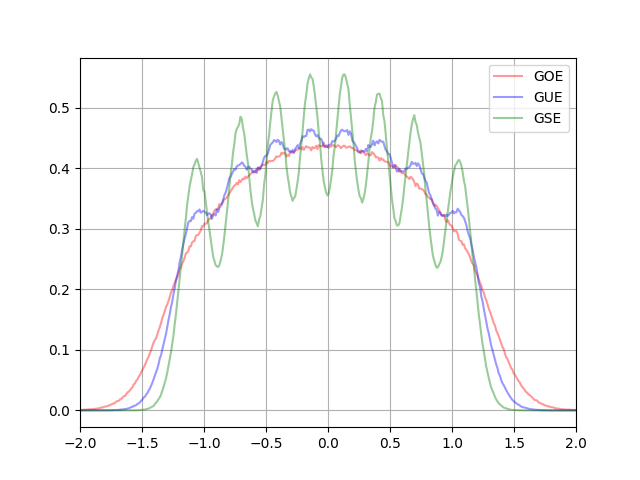
\includegraphics[width=0.8\linewidth]{FullGaussianDensityEscaled.png}
	\label{fig: lambdadist}
\end{center}

Mais desenvolvimento sobre a forma desta distribuição e as diferenças será feito posteriormente. Usaremos a referência \cite{Livan_2018} para a maior parte dos desenvolvimentos. Algum material interessante pode ser consultado em um livro de física em \cite{MEHTA1967v}.

\section{Termodinâmica}
Estaremos lidando o tempo todo no nosso estudo com funções partições, de alguma forma, compartilhada com a física. Entenderemos um pouco mais sobre os desenvolvimentos do ensemble canônico na termodinâmica.


\subsection{Uma abordagem mais física}

Para o desenvolvimento da função partição estamos atentos aos requisitos do ensemble canônico. Um sistema termalizado por um banho térmico. Nosso sistema completo pode ser representado

\begin{center}
	\begin{tikzpicture}
		\fill[blue!10!white] (0,0) rectangle (8,3);
		\draw (0,0) rectangle (8,3);
		\fill[green!10!white] (0,0) rectangle (2,3);
		\draw (0,0) rectangle (2,3);
		\node at (1,2) {$\mathcal{S}$};
		\node at (1,0.5) {$E$};
		\node at (5,2) {$\mathcal{S}_r$};
		\node at (7.5,0.5) {$T$};
		\node at (3,0.5) {$E_t - E$};
	\end{tikzpicture}
\end{center}

Considere que os sistemas estão em contato térmico e o sistema completo, junto com o banho é um sistema isolado de energia $E_t$. Sabemos que a probabilidade de uma energia no nosso sistema termalizado ($\rho_E$) é expressa:

\[
	\rho_E = \sum_{\sigma} \rho_\sigma = \Omega(E)\rho_\sigma
\]

Onde note, $\rho_\sigma$ é a probabilidade de, dada uma temperatura, um microestado possível. Note por outro lado que podemos expressar:

\[
	\rho_E = \frac{\Omega(E) \Omega_r (E_t - E)}{\sum_{i} \Omega(E_i) \Omega_r(E_t-E)}
\]

Note que isso é nada mais do que dizer que os microestados são equiprováveis e basta uma contagem (normalizada) para definir a probabilidade. Neste sentido podemos também escrever:

\[
	\rho_\sigma \propto \Omega_r(E_t - E)
\]

Isso é, quanto mais formas o reservatório possa se organizar para determinada energia, mais provável é o microestado associado à energia de $\mathcal{S}$.

\begin{align*}
	\rho_\sigma & \propto e^{\beta T K_b \log{(\Omega_r(E_t - E))}} \\
				& \propto e^{\beta T \left( \mathcal{S}_r(E_t) - \frac{E}{T}\right) } \\
				& \propto e^{-\beta E} e^{\beta T \mathcal{S}_r(E_t)} \\
				& \propto e^{-\beta E}
\end{align*}

Onde fizemos a expansão de $k_b \log{(\Omega_r(E_t - E))}$ (entropia) em Taylor (apesar de que, em realidade, apenas $\frac{E}{E_t}$ é pequeno, não necessariamente $E$) e obtemos

\[
	\mathcal{S}_r(E_t - E) \approx \mathcal{S}_r(E_t) + \left( \frac{\partial \mathcal{S}_r}{\partial E}\right)_{E=E_t} (-E)
\]

Onde 

\[
	\left( \frac{\partial \mathcal{S}_r}{\partial E} \right)_{E=E_t} = \frac{1}{T}
\]

\subsection{A entropia de Shannon}

Podemos fazer algo um pouco mais matemático. Definiremos a entropia de Shannon

\[
	\mathcal{S} = -k_b \sum_{i} p_i \log{p_i}
\]

\subsubsection{Um vínculo}

Se impormos um vínculo do tipo

\[
	\sum_{i} p_i = 1
\]

Podemos usar os multiplicadores de Lagrange para realizar a maximização da nossa função. Pela definição, escrevemos:

\[
	S({p_i}, \lambda) \equiv k_b \sum_{i=1}^{N} p_i \log{(p_i)} - \lambda \left( \sum_{i=1}^{N}p_i -1 \right) 
\]

Com diferencial

\[
	\delta S = - k_b \sum_{i=1}^{N} \left( p_i \log{p_i} + \frac{p_i}{p_i} \delta p_i \right) - \lambda \sum_{i=1}^{N}\delta p_i
\]

Resolveremos agora o sistema

\[
 \begin{cases}
	\delta S = 0 \\
	\sum_{i} p_i = 1
\end{cases}
\]

ou seja,

\[
\begin{cases}
	-k_b (\log{p_i} + 1) - \lambda \\
	\sum_{i} p_i = 1
\end{cases}
\]

Note que $p_i = cte \ \forall i$. Teremos então $p_i = \frac{1}{N}$. A entropia neste caso será 

\[
	S({p_i}^*) = - k_b \sum_{i=1}^{N} \left( \frac{1}{N} \log{\frac{1}{N}} \right) = k_b \log{N}
\]

\subsubsection{Dois vínculos}

Faremos agora a implicação de um novo vínculo

\[
\sum_{\sigma} p_\sigma E_\sigma = U
\]

Desenvolvendo a equação

\[
S({p_i}, \lambda) \equiv k_b \sum_{i=1}^{N} p_i \log{(p_i)} - \lambda_1 \left( \sum_{i=1}^{N}p_i -1 \right)  - \lambda_2 \left( \sum_\sigma  p_\sigma E_\sigma - U \right) 
\]

Chegaremos no sistema


\[
\begin{cases}
	-k_b (\log{p_i} + 1) - \lambda_1 - \lambda_2 E_\sigma \\
	\sum_{\sigma} p_i = 1 \\
	\sum_{\sigma} p_\sigma E_\sigma = U
\end{cases}
\]

E finalmente, da primeira equação tiramos

\[
	p_\sigma = e^{A E_\sigma + B} = M e^{-\beta E_\sigma}
\]

De forma que podemos reescrever

\[
	1 = \sum_\sigma M e^{-\beta E_\sigma} = M \sum_\sigma e^{-\beta E_\sigma}
\]

Onde nomearemos $M = \frac{1}{\sum_{\sigma}e^{-\beta E_\sigma}} = \frac{1}{\mathcal{Z}}$ \textbf{função partição}. Falta apenas definir $\beta$ em

\[
	p_\sigma = \frac{e^{-\beta E_\sigma}}{Z}
\]

Para $\beta$ podemos aplicar o último vínculo (da temperatura térmica)

\[
	U = \sum_\sigma p_\sigma E_\sigma = \sum_\sigma \left( \frac{1}{Z} e^{-\beta E_\sigma} \right) E_\sigma = \frac{1}{Z} \sum_\sigma E_\sigma e^{-\beta E_\sigma}
\]

\[
	-\frac{1}{Z} \frac{\partial }{ \partial \beta} \left( \sum_\sigma e^{-\beta E_\sigma} \right) = -\frac{1}{\mathcal{Z}} \frac{\partial Z}{\partial \beta} = - \frac{\partial (\log{Z})}{\partial \beta}
\]

De alguma forma esta equação transcendental nos define $\beta$.




\section{Porquê exponencial?}
\subsection{Shannon-Quem?}

O uso da p.d.f gaussiana pode ser justificado de algumas formas. Uma primeira abordagem a ser explorada é a de maximização entrópica ou minimização de informação similar aos trabalhos de Shannon-Kinchin. Definiremos uma grandeza $\mathcal{I}[\mathcal{P}(\matriz{H})]$ associada à uma p.d.f tal que:

\[
	\mathcal{I}[\mathcal{P}(\matriz{H})] = - \int d\mu (\matriz{H}) \mathcal{P}(\matriz{H}) \ln{\mathcal{P}(\matriz{H})} 		
\]

Que é uma extensão natural da definição discreta de informação $- \sum_{l=1}^{m} p_m \ln{p_m}$. Agora argumentaremos algo parecido com os argumentos usados em termodinâmica de maximização de entropia. Diremos que a incerteza sobre as matrizes será máxima, ou seja, teremos a maior aleatoriedade das matrizes quando a entropia for maximizada e a informação, minimizada. Assim como na entropia física impomos um vínculo de energia constante, aqui faremos algo do tipo $E(\Tr{\matriz{H}}) = b$ e $E((\Tr{\matriz{H}})^2) = a > 0$. Vamos introduzir esses vinculos como multiplicadores de lagrange com multiplicadores $v_1$ e $v_2$. 

\[
	\mathcal{I}[\mathcal{P}(\matriz{H})] = - \int d\mu (\matriz{H}) \mathcal{P}(\matriz{H}) \left( \ln{\mathcal{P}(\matriz{H})} - v_1 \Tr{\matriz{H}} - v_2 \Tr{\matriz{H}}^2 \right)	
\]	

que tem diferencial

\[
\delta \mathcal{I}[\mathcal{P}(\matriz{H})] = - \int d\mu (\matriz{H})  \delta \mathcal{P}(\matriz{H}) \left( 1 + \ln{\mathcal{P}(\matriz{H})} - v_1 \Tr{\matriz{H}} - v_2 \Tr{\matriz{H}}^2 \right)	= 0
\]

Que só vai ser mínimo se 

\[
	\mathcal{P}(\matriz{H}) \propto e^{ - v_1 \Tr{\matriz{H}} - v_2 \Tr{\matriz{H}}^2}
\]

Onde os multiplicadores são unicamente definidos pelas constantes do vínculo. Esse fato motiva de alguma forma o estudo da p.d.f gaussiana para as matrizes.

\section{Independência ou Morte}
Consideremos matrizes com entradas independentes. Qual a função densidade de probabilidade (F.P.D.) da matriz simétrica $\matriz{H_s}$? Devemos fazer separadamente a diagonal da seção triangular que formos usar e teremos

\[
\rho((\matriz{H_s})_{11}, \dots, (\matriz{H_s})_{NN}) = \prod_{i=1}^{N} \left[ \frac{e^{\frac{-(H_s)^2_{ii}}{2}}}{2\pi} \right] \prod_{i<j} \left[ \frac{e^{-(H_s)^2_{ij}}}{\sqrt{\pi}} \right]
\]

Podemos também definir a distribuição para os autovalores de uma matriz Gaussiana de dimensão $N$ como \footnote{Esse resultado é não óbvio e deve ser discutido em breve.}

\begin{equation}
	\rho(x_1, \dots, x_N) = \frac{1}{\mathcal{Z_{N, \beta}}} e^{-\frac{1}{2} \sum_{i=1}^{N} x_i^2} \prod_{j<k} | x_j - x_k |^{\beta}
\end{equation}

onde a constante de normalização é dada por

\[
\mathcal{Z_{N, \beta}} = (2\pi)^\frac{N}{2} \prod_{j=1}^{N} \frac{\Gamma(1+ j\frac{\beta}{2})}{\Gamma(1+ \frac{\beta}{2})}
\]

Para ressaltar um pouco do jargão, $\beta$ é denominado \textit{Dyson Index} que em suma se refere à "dimensão" das suas entradas na matriz. $1$ para GOE, $2$ para GUE e $4$ para GSE.

Algumas observações sobre essa expressão são interessantes. Note que o fator exponencial deve matar qualquer chance de uma matriz com autovalor alto. Ao mesmo tempo o fator de dependência deve matar qualquer configuração com autovalores muito próximos entre si. Existe um efeito de repelência entre autovalores na expressão.

\section{Uma medida à Hermitiana}
Consideraremos no nosso estudo para referencia matrizes quadradas de entradas complexas com dimensão $N$. Nosso objetivo é afinal ter uma forma de mensurar a distribuição de autovalores e para isso, faremos os seguintes desenvolvimentos.

Consideremos inicialmente um espaço de matrizes com entradas complexas $2N^2$ dimensional. Contido neste espaço temos um espaço de maior interesse correspondente ao espaço das matrizes \textit{hermitianas} de dimensão $N^2$. A escolha do subespaço está relacionada com o fato que matrizes hermitianas são diagonalizáveis e a distribuição de seus autovalores estará diretamente relacionada (com uma mudança de base) à distribuição do traço da matriz diagonalizada. Note que para a matriz diagonal ter a mesma medida que nossa matriz inicial, nossa medida deve ser invariável por rotação.

Mais detalhadamente podemos escrever nossa matriz hermitiana $\matriz{H}$ como 

\[
\matriz{H} = \matriz{U} \matriz{\Lambda} \matriz{U}^{-1} \ , \ \matriz{\Lambda} = diag(\lambda_1, \dots, \lambda_2) \ , \ \matriz{U}\cdot\matriz{U}^* = I
\]

onde, claro, $\matriz{\Lambda}$ é diagonal de autovalores e $\matriz{U}$ é unitária e com colunas equivalentes aos autovetores de $\matriz{H}$. Em geral, o conjunto de matrizes degeneradas tem medida nula e não é uma preocupação. Um cuidado deve ser tomado. A correspondência $\matriz{H} \implies (\matriz{U} \ U(N), \matriz{\Lambda})$ não é injetora, podemos tomar $\matriz{U}_1 \matriz{\Lambda} \matriz{U}_1^{-1} = \matriz{U}_2 \matriz{\Lambda} \matriz{U}_2^{-1}$ se $\matriz{U}_1^{-1} \matriz{U}_2 = diag(e^i\phi_1, \dots, e^i\phi_N)$ para qualquer escolha de fases $(\phi_1, \dots, \phi_N)$. Para restringir nosso problema e tornar a função injetiva será necessário considerar as matrizes unitárias ao espaço de coset $U(N) / U(1) \times \dots \times U(1)$ \footnote{Não tenho muita ideia de espaços de Coset. Pelo que entendo, existe um espaço onde toda $\matriz{U}$ pode ser representada por $\matriz{U}_c \matriz{U}_d$, onde $\matriz{U}_c$ compõe o espaço de coset e $\matriz{U}_d$ é uma matriz diagonal unitária. Dessa forma matrizes equivalentes são aquelas que multiplicadas por $\matriz{U}_d$ tem um mesmo resultado.}. Uma outra restrição necessárias é ordenas os autovalores, ou seja, $\lambda_1 < \dots < \lambda_n$. Temos que reescrever agora a medida $d\mu(\matriz{H})$ em função de auvalores e da $\matriz{U}$ de autovetores.

Para resumir o desenvolvimento, alguns resultados serão diretamente enunciados. Essa seção pode ser encontrada no relatório \cite{fyodorov2010introduction}. Em especial recuperaremos o elemento de distância e volume no subespaço que vamos tratar

\begin{equation}
	(ds)^2 = \Tr{d\matriz{H} d\matriz{H}^*} = \sum_{i} (dx_{ii})^2 + 2 \sum_{i < j} \left[(dx_{ij})^2 + (dy_{ij})^2 \right]
	\label{eq: ds}
\end{equation}

\begin{equation}
	d\mu(\matriz{H}) = 2^{\frac{N(N-1)}{2}} \prod_{i} dx_{ii} \prod_{i<j} dx_{ij} dy_{ij}
	\label{eq: du}
\end{equation}

Ambos vem de um desenvolvimento da métrica do espaço discutido. Note que nossa medida de comprimento é invariante em respeito à automorfismos. Especificamente, se tomarmos os elementos \eqref{eq: ds} e \eqref{eq: du} na decomposição espectral, obteremos

\begin{equation}
	(ds)^2 = \sum_{i} (d\lambda)^2 + \sum_{i<j} (\lambda_i - \lambda_j)^2 \overline{\delta U_{ij}} \delta U_{ij}
\end{equation}

e

\begin{equation}
	d\mu(\matriz{H}) = \prod_{i < j} (\lambda_i - \lambda_j)^2 \prod_{i} d\lambda_i \times d\mu(\matriz{U})
\end{equation}

Tendo a medida de integração pronta, podemos definir uma F.D.P $\mathcal{P}(\matriz{H})$ neste espaço de matizes hermitianas tal que $\mathcal{P}(\matriz{H}) d\mu(\matriz{H})$ é a probabilidade da matriz $\matriz{H}$  estar no volume $d\mu(\matriz{H})$. Queremos que nossa função seja invariante à rotação, ou seja, $\mathcal{P}(\matriz{H}) = \mathcal{P}( \matriz{U}^* \matriz{H} \matriz{U})$.

Conhecer os $N$ primeiros traços ($\Tr{\matriz{H}^n}$) de $\matriz{H}$ define unicamente o polinômio característico e junto com ele, os autovalores. Especificamente tomaremos 

\begin{equation}
	\mathcal{P}(\matriz{H}) = Ce^{-\Tr{Q(\matriz{H})}}
	\label{eq: p}
\end{equation}

Onde $Q$ deve ser um polinômio de até ordem $2j \leq N$ suficiente para garantir a convergência de

\[
	\mathcal{Z}_n = \int_{\mathcal{H}_n} e^{-\Tr{Q(\matriz{M})}} d\matriz{M} 
\]

Comumente uma condição suficiente é

\[
	\lim_{x \rightarrow \pm \infty} \frac{Q(x)}{\ln{(1+x^2)}} = \infty
\]

Mas em especial, se tomarmos

\[
	Q(x) = ax^2 + bx + c
\]


Nossa medida tomará a forma

\begin{align}	
	\mathcal{P}(\matriz{H}) & = e^{-a \left[ \sum_{i} x_{ii}^2 + 2 \sum_{i < j} [x_{ij}^2 + y_{ij}^2] \right] } e^{-b \sum_{i} x_{ii}} e^{-c N} \\
	& = e^{-cN} \prod_{i=1}^{N} \left( e^{-ax^2_{ii}-bx_{ii}} \right) \prod_{i<j} e^{-2ax^2_{ij}} \prod_{i<j} e^{-2ay^2_{ij}}
\end{align}

Onde podemos notar que a distribuição de probabilidade da matriz $\matriz{H}$ pode ser representados por fatores independentes, cada um de forma gaussiana. Para este potencial, temos uma conexão entre as matrizes de entrada independentes e as matrizes invariáveis por rotação. Lembre-se que para as variáveis serem independentes $\mathcal{P}$ deve ter a forma $\mathcal{P} = Ce^{-\left( a\Tr{\matriz{H}^2} + b\Tr{\matriz{H}} + cN \right)}$ para constantes $a>0, b, c$. Em nota, sabemos então

\[
e^{\Tr{V(\matriz{H})}}  d\mu(\matriz{H}) = e^{-\sum_{j} V(\lambda_j)}  \prod_{i < j} (\lambda_i - \lambda_j)^2 d\mu(\lambda) d\mu(\matriz{U})
\]

ou mais geralmente para o ensemble com 

\[
	\frac{1}{{\mathcal{\tilde{Z}}}_n} e^{\Tr{(V(\matriz{M}))}} dM
\]

Dado $\lambda_j$ os autovalores

\[
	\Tr{(V(\matriz{M}))} = -\sum_{j=1}^{n} V(\lambda_j)
\]

e finalmente podemos escrever

\begin{align}
	E[f]& = \int_{\mathcal{H}_n} f(\matriz{M}) e^{-\Tr{(Q(\matriz{M}))}} d\matriz{M} \\
	&  = \frac{1}{\mathcal{Z}} \int \dots \int f(\lambda_1, \dots, \lambda_n) \prod_{i < j} (\lambda_i - \lambda_j)^2 \prod_{j=1}^{n} e^{-Q(\lambda_j)} d\lambda_1 \dots d\lambda_n
\end{align}

Assim, a probabilidade conjunta nas matrizes induz uma densidade de probabilidade de autovalores

\[
	\frac{1}{\mathcal{Z}_n} \prod_{i<j} (\lambda_i - \lambda_j)^2 \prod_{j=1}^{n} e^{Q(\lambda_j)}
\]

Alguns resultados foram resgatadas da nota do autor em \cite{ArnoLectureNotes}.{\tiny }

\chapter{Movimento Browniano}
\input{chapters/brownian}

\section{Processo Pontual}
Um processo pontual pode ser interpretado como um conjunto aleatório de pontos ou como a medida de probabilidade associada a esse conjunto. Um processo pontual possui $n$ pontos se

\[
\mathcal{P}(\# X=n) = 1
\]

Onde $X$ é um conjunto enumerável de $\mathcal{X}$ ($\mathbb{R}$, $\mathbb{Z}$ ou um subconjunto destes). O conjunto de todas configurações possíveis é denominado $Conf(\mathcal{X})$. Se $P(x_1, \dots, x_n)$ é uma função de densidade de probabilidade em $\mathbb{R}^n$ invariante por permutações

\[
	\mathbb{R}^n \rightarrow Conf(\mathbb{R})
\]
\[
	(x_1, \dots, x_n) \mapsto X = {x_1, \dots, x_n}
\]

define naturalmente um processo pontual com $n$ pontos.

\subsection{Poisson \& fries}

Tome $\set{N(t)}$ o número de eventos no intervalo de tempo $]0,t]$. $\set{N(t)}$  é um processo estocástico (de contagem). Se o processo de Poisson possui $\lambda > 0$, para um elemento fiox do espaço amostral a variável aleatória $N$ assume valor $k$ no tempo $t$ com probabilidade

\begin{equation}
	\mathcal{P}[N(t) = k] = \frac{(\lambda t)^k e^{-\lambda t}}{k!}
\end{equation}

Onde $\lambda$ é o número esperado de chagadas por unidade de tempo. Agora, como um processo pontual, a probabilidade de n eventos no intervalo $]a,b]$ é

\[
	\mathcal{P}(N]a,b] = n) =  \frac{(\lambda (b-a))^n e^{-\lambda (b-a)}}{n!}
\]

Podemos usar a independência de cada evento de Poisson em intervalos disjuntos para escrever

\[
	\mathcal{P}(N]a_1,b_1] = n_1, \dots, N]a_k,b_k] = n_k) = \prod_{i=1}^{k} \frac{(\lambda (b_i-a_i))^n_i e^{-\lambda (b_i-a_i)}}{n_i!}
\]

Podemos escrever para uma função $f$ mensurável em $\mathbb{R}$

\[
	\sum_{x_i \in \mathcal{X}} f(x_i) = \int f(x) dN(x)
\]

Onde a medida dN é

\[
	dN(x) = \sum_{x_i \in \mathcal{X}} \delta_{x_i} (x)
\]

Onde notamos que podemos interpretar tanto quanto uma soma de um processo pontual quanto uma medida de probabilidade.


\subsection{Funcão Correlação}

Definimos uma variável aleatória $N$ anteriormente. Naturalmente, poderíamos estar interessados em sua esperança. Mais especificamente, podemos procurar a esperança do número de pontos de uma ocnfiguração dentro de um intervalo $A \subset \mathbb{R}$.

\[
	A \mapsto \mathbb{E}[N(A)] = \mathbb{E}[\#(A \cap X)]	
\]

Que pode ser interpretada como uma medida com densidade $p_1$

\begin{equation}
	\mathbb{E}[\#(A \cap X)] = \int_{A} p_1(x) dx
	\label{eq: p1}
\end{equation}

A equação \ref{eq: p1} é conhecida como \textit{função de correlação de 1 ponto}. Em grosso modo, $p_1(x)$ é a probabilidade de haver um ponto da configuração entre $x$ e $x+dx$. Seja um configuração simples $X = \set{x_1, \dots, x_n}$ e intervalos disjuntos na reta \many{A}{n},

\[
	\int_A \dots \int_A \rho_n(x_1, \dots, x_n) dx_1, \dots, dx_n = \mathbb{E} \left( \prod_{j=1}^{k} \# (X \cap A_j) \right) 
\]

é o número esperado de n-uplas (\many{x}{n}) $\in A_1 \times \dots \times A_n$ tais que $x_i \in A_i, i=1,\dots,n$. Seja $\mathbb{P}(x_1, \dots, x_n)$ uma densidade de probabilidade em $\mathbb{R}^n$, então o processo pontual de n pontos gerado possui funções de correlação dadas por

\[
	p_k(x_1, \dots, x_k) = \frac{n!}{(n-k)!} \int \dots \int \mathbb{P}(x_1, \dots, x_n) dx_{k+1}\dots dx_n
\]


\subsection{Pontual Determinantal}

Um processo pontual vai ser chamado determinantal se dada uma função de correlação $\rho_n$, existe um núcleo $K(x, y)$ conhecido como núcleo de correlação tal que

\begin{equation}
	\rho_n(x_1, \dots, x_n) = det[K(x_i, x_j)]_{i,j=1}^{n}
	\label{eq: pontualdet}
\end{equation}

onde

\[
[K(x_i,x_j)]_{i,j=1}^{n} = 
\begin{bmatrix}
	K(x_1, x_1) & K(x_1, x_2) & \dots & K(x_n, x_n) \\
	K(x_2, x_1) & K(x_2, x_2) & \dots & K(x_n, x_n) \\
	\vdots & \vdots & \ddots & \vdots \\
	K(x_n, x_1) & K(x_n, x_2) & \dots & K(x_n, x_n)
\end{bmatrix}
\]

Nos casos de baixa dimensão

\[
p_1(x_1) = K(x_1,x_1), \quad \quad p_2(x_1,x_2) =
\begin{vmatrix}
	K(x_1, x_1) & K(x_1, x_2) \\
	K(x_2, x_1) & K(x_2, x_2)
\end{vmatrix}
\]

Para que o núcleo satisfaça a equação \ref{eq: pontualdet} enunciaremos um resultado de interesse.

\begin{theorem}
	Seja K um núcleo tal que
	\begin{enumerate}[label=(\alph*)]
		\item $\int K(x,x) = n \in \mathbb{N}$,
		\item Para todo \many{x}{n} $\in \mathbb{R}$, o determinante é não negativo
		\item K possui a propriedade de \textbf{núcleo reprodutor}, isto é;
		\[
		K(x,y) = \int_{-\infty}^{\infty} K(x,s) K(s,y) ds
		\]
		Então
		\[
		P(x_1,\dots, x_n) = \frac{1}{n!} det[K(x_i, x_j)]_{i,j=1}^{n}
		\]
		será uma densidade de probabilidade em $\mathbb{R}$ cujo processo de n pontos associado é determinantal.
	\end{enumerate}
\end{theorem}



\section{Emsemble Biortogonal}
Um n-ponto processo é um ensemble biortogonal se existem duas sequências $f_1, \dots, f_n$ e $g_1, \dots g_n$ em $L^2(R)$ e uma constante $\mathcal{Z}_n \neq $ tais que:

\[
	\mathcal{P}(x_1, \dots, x_n) = \frac{1}{\mathcal{Z}_n} \det{[f_i(x_j)]_{i,j=1}^{n}} \cdot \det{[g_i(x_j)]_{i,j=1}^{n}}
\]

Onde todo $f_i$ e $g_i$ é independente nos $i$'s. Pode-se mostrar que se

\[
	\phi_j \in span(f_1, \dots, f_n) \ \ \psi_j \in span(g_1, \dots, g_n)
\]

tais que 

\[
	\int_{-\infty}^{\infty} \phi_k(c) \psi_j(x) dx = \delta_{jk}
\]

então

\[
	K_n(x,y) = \sum_{j=1}^{n} \phi_k(c) \psi_j(x)
\]

onde $K_n(x, y)$ é um \textit{Kernel} tal que

\[
	\mathcal{P}(x_1, \dots, x_n) = \frac{1}{n!} \det{[K_n(x_i, x_j)]_{i,j=1}^{n}}
\]

O processo é determinado e $K_n$ é o kernel de correlação.

\section{Karlin-McGregor}
\subsection{O teorema}

Exploraremos os caminhos não cruzantes providos por processos de Markov. Considere uma partícula de movendo com uma regra qualquer, vamos descrever esse movimento de forma que denotaremos $p_t(a;x)$ a densidade de probabilidade de transição; isto é, a chance uma partícula em $a$ ir para $x$ em um próximo momento. Um teorema clássico enuncia a probabilidade de um certo número de caminhos não se intersectarem passado um tempo $t$.

O teorema diz: Considere $X_1(t), \dots, X_n(t)$ cópias independentes de um processo forte de Markov com caminhos condicionados tais que

\[
	X_j(0) = a_j
\] 

onde \cmany{a}{n}{<} são valores dados. Notamos novamente $p_t(x, y)$ ser a densidade do processo de transição. Vamos definir regiões \many{E}{n} onde $E$'s vizinhos não se intersectam. Temos

\[
	\int_{E_1} \dots \int_{E_n} \det{[p_t(a_i, x_j)]^{n}_{i,j=1}} dx_1 \dots dx_n
\]

vai ser a probabilidade de que os caminhos não tenham se intersectados no intervalo de tempo $[0, t]$ e $X_j(t)$ nos intervalos correspondentes. A demonstração está em \cite{ArnoLectureNotes}. Note que temos

\[
\int_{E_1} \dots \int_{E_n} \det{[p_t(a_i, x_j)]^{n}_{i,j=1}}  dx_1 \dots dx_n
\]

\begin{align}
	& = \int_{E_1} \dots \int_{E_n}
	\begin{vmatrix}
		p_t(a_1, x_1) 	& p_t(a_2, x_1) 	 & \dots	& p_t(a_{n-1}, x_1) 	& p_t(a_n, x_1) \\
		p_t(a_1, x_2) 	& p_t(a_2, x_2) 	 & \dots 	&  p_t(a_{n-1}, x_2)				&  p_t(a_n, x_2) \\
		\vdots 			& \vdots 			 & \vdots 	& \vdots 				& \vdots \\
		p_t(a_1, x_{n-1}) & p_t(a_2, x_{n-1})& \dots 	&  	p_t(a_{n-1}, x_{n-1})	& p_t(a_n, x_{n-1}) \\
		p_t(a_1, x_n) 	& p_t(a_2, x_n) 	 & \dots  	& p_t(a_{n-1}, x_n) 	& p_t(a_n, x_n)
	\end{vmatrix} dx_1 \dots dx_n \\ 
	& = \sum_{\sigma}sgn(\sigma) \prod_{j=1}^{n} p_t(a_j, E_{\sigma(j)}) \\
	& = \sum_{\sigma} sgn(\sigma) \mathcal{P}(A_\sigma)
	\label{eq: detInd}
\end{align}

Onde denotamos

\[
	p_t(a_j, E_{\sigma(j)}) = \int_{E_j} p_t(a_i, x_j) dx_j
\]

$\sigma$ é uma permutação de ${1, \dots, n}$ e $A_{\sigma}$ é o evento que $X_j(t) \in E_{\sigma(j)}$ para todo $j$. Os caminhos devem ser independentes para \ref{eq: detInd}.

De alguma forma o determinada permuta os caminhos em todas ordens possíveis e calcula a probabilidade de todos se manterem nos intervalos adequados. Um exemplo de baixas dimensões pode mostrar que


\begin{align}
	&
	\begin{vmatrix}
		p_t(a_1, x_1) & p_t(a_2, x_1) & p_t(a_3, x_1) \\
		p_t(a_1, x_2) & p_t(a_2, x_2) & p_t(a_3, x_2) \\
		p_t(a_1, x_3) & p_t(a_2, x_3) & p_t(a_3, x_3)
	\end{vmatrix} =\\
	&
	+ p_t(a_1, x_1) p_t(a_2, x_2) p_t(a_3, x_3)  \\
	&
	+ p_t(a_2, x_1) p_t(a_3, x_2) p_t(a_1, x_3) \\
	&
	+ p_t(a_3, x_1) p_t(a_1, x_2) p_t(a_2, x_3) \\
	& 
	- p_t(a_3, x_1) p_t(a_2, x_2) p_t(a_1, x_3) \\
	&
	-  p_t(a_2, x_1) p_t(a_1, x_2) p_t(a_3, x_3) \\
	&
	- p_t(a_1, x_1) p_t(a_3, x_2) p_t(a_2, x_3)
\end{align}

Logo

\begin{align}
	\int_{E_1} \dots \int_{E_n} \det{[p_t(a_i, x_j)]^{n}_{i,j=1}}  dx_1 \dots dx_n  = 
	&
	+ p_t(a_1, E_1) p_t(a_2, E_2) p_t(a_3, E_3)  \\
	&
	+ p_t(a_2, E_1) p_t(a_3, E_2) p_t(a_1, E_3) \\
	&
	+ p_t(a_3, E_1) p_t(a_1, E_2) p_t(a_2, E_3) \\
	& 
	- p_t(a_3, E_1) p_t(a_2, E_2) p_t(a_1, E_3) \\
	&
	-  p_t(a_2, E_1) p_t(a_1, E_2) p_t(a_3, E_3) \\
	&
	- p_t(a_1, E_1) p_t(a_3, E_2) p_t(a_2, E_3)
\end{align}

Onde somamos os casos onde as partículas se matém ordenadas e subtraímos os casos onde elas se cruzam.


\subsection{Consequências}

Considere $n$ cópias do processo de Markov condicionado para começar em $t=0$ nas determinadas posições \cmany{a}{n}{<}. Se condicionarmos estes processos para não intersectar no intervalo $[0,t]$, o teorema vai nos dizer que os caminhos em um tempo $t$ vão ter uma densidade de probabilidade conjunta

\[
	\frac{1}{\mathcal{Z}_n} \det{[p_t(a_i, x_j)]^{n}_{i,j=1}}
\]

Mas este não pode ser considerado um processo pontual determinado. Não é expresso por um produto de determinantes. Isso pode ser ajeitado se considerarmos um tempo $T > t$ no nosso processo. Tomaremos \many{b}{n} posições finais e condicionaremos os caminhos a não intersectar no intervalo $[0, T]$ com $X_j(0) = a_j$ e $X_j(T) = b_j$ para todos. É possível mostrar que a distribuição conjunta deles será

\[
	\frac{1}{\mathcal{Z}_n'} \det{[p_t(a_i, x_j)]^{n}_{i,j=1}} \det{[p_{T-t}(x_i, b_j)]^{n}_{i,j=1}}
\]

Que será biortogonal com as funções

\[
	f_j = p_t(a_j, x) \ ; \ g_j = p_{T-t}(x, b_j)
\]

E nosso caso de interesse é quando $a_j \rightarrow a$ e $b_j \rightarrow b$. Note que usando as duas funções podemos forçar que o movimento browniano se inicie em um ponto e encerre em outro determinado. Em uma, reverteremos o tempo e, nos limites $0$ e $T$, forçaremos que apenas uma das funções seja predominante de forma que a posição inicial de cada uma prevaleça. Podemos impor a posição inicial e final do movimento. No caso browniano teremos

\[
	p_t(a, x) = \frac{1}{\sqrt{2\pi t}} e^{-\frac{(x-a)^2}{2t}}
\]

No caso dos limites de $a$ e $b$ ficamos com

\[
	f_j = F_{j-1}(x)e^{-\frac{(x-a)^2}{2t}} \ ; \ g_j = G_{j-1}(x)e^{-\frac{(x-b)^2}{2(T-t)}}
\]

onde $F$ e $G$ são polinômios em $x$  de grau $j-1$. Este processo podemos escalar e transladar para uma versão do GUE $n \times n$.





\chapter{Chapter Two Title}
\input{chapters/chapter02}

\chapter{Chapter Three Title}
\input{chapters/chapter03}

\chapter{Chapter Four Title}
\input{chapters/chapter04}

\chapter{Conclusion}
\input{chapters/conclusion}

\bibliography{references}{}
\bibliographystyle{plain}

\appendix
\chapter{Appendix Title}
\input{chapters/appendix}


\end{document}          
